%%%%%%%%%%%%%%%%%%%%%%%%%%%%%%%%%%%%%%%%%
% Simple Sectioned Essay Template
% LaTeX Template
%
% This template has been downloaded from:
% http://www.latextemplates.com
%
% Note:
% The \lipsum[#] commands throughout this template generate dummy text
% to fill the template out. These commands should all be removed when 
% writing essay content.
%
%%%%%%%%%%%%%%%%%%%%%%%%%%%%%%%%%%%%%%%%%

%----------------------------------------------------------------------------------------
%	PACKAGES AND OTHER DOCUMENT CONFIGURATIONS
%----------------------------------------------------------------------------------------

\documentclass[11pt]{article} % Default font size is 12pt, it can be changed here

\usepackage{geometry} % Required to change the page size to A4
\geometry{a4paper} % Set the page size to be A4 as opposed to the default US Letter

\usepackage{graphicx} % Required for including pictures

\usepackage{float} % Allows putting an [H] in \begin{figure} to specify the exact location of the figure
\usepackage{wrapfig} % Allows in-line images such as the example fish picture

\usepackage{lipsum} % Used for inserting dummy 'Lorem ipsum' text into the template

\linespread{1.0} % Line spacing

%\setlength\parindent{0pt} % Uncomment to remove all indentation from paragraphs

\graphicspath{{Pictures/}} % Specifies the directory where pictures are stored

\usepackage[
sorting=none,
minbibnames=8,
maxbibnames=9,
block=space,
backend=biber
]{biblatex}
\bibliography{export}

\begin{document}

%----------------------------------------------------------------------------------------
%	TITLE PAGE
%----------------------------------------------------------------------------------------

%\begin{titlepage}
%
%\newcommand{\HRule}{\rule{\linewidth}{0.5mm}} % Defines a new command for the horizontal lines, change thickness here
%
%\center % Center everything on the page
%
%\textsc{\LARGE University Name}\\[1.5cm] % Name of your university/college
%\textsc{\Large Major Heading}\\[0.5cm] % Major heading such as course name
%\textsc{\large Minor Heading}\\[0.5cm] % Minor heading such as course title
%
%\HRule \\[0.4cm]
%{ \huge \bfseries Title}\\[0.4cm] % Title of your document
%\HRule \\[1.5cm]
%
%\begin{minipage}{0.4\textwidth}
%\begin{flushleft} \large
%\emph{Author:}\\
%John \textsc{Smith} % Your name
%\end{flushleft}
%\end{minipage}
%~
%\begin{minipage}{0.4\textwidth}
%\begin{flushright} \large
%\emph{Supervisor:} \\
%Dr. James \textsc{Smith} % Supervisor's Name
%\end{flushright}
%\end{minipage}\\[4cm]
%
%{\large \today}\\[3cm] % Date, change the \today to a set date if you want to be precise
%
%%\includegraphics{Logo}\\[1cm] % Include a department/university logo - this will require the graphicx package
%
%\vfill % Fill the rest of the page with whitespace
%
%\end{titlepage}

%----------------------------------------------------------------------------------------
%	TABLE OF CONTENTS
%----------------------------------------------------------------------------------------

%\tableofcontents % Include a table of contents
%
%\newpage % Begins the essay on a new page instead of on the same page as the table of contents 

%----------------------------------------------------------------------------------------
%	INTRODUCTION
%----------------------------------------------------------------------------------------

\section*{WS1-4, Question 5, Object Oriented Design} % Major section
Author: Thomas Brereton\\
ID number: 1708846
\newline


%------------------------------------------------

In this question we are asked to explain ``the rationale for the use of object oriented programming'' This question can be broken down into the following points.

\begin{itemize}
	\item What problems does object oriented programming solve
	\item How does it solve these problems
	\item To what degree does it solve these problems
\end{itemize}

Object oriented programming (OOP) is an evolution in programming and attempts to provide an effective style of code. Object oriented design consists of the principles;  Classes, Objects, Encapsulation and Abstraction of Information, Inheritance, and Polymorphism. These principles try to address known software engineering problems by enabling the key features\cite{deitel:1}:

\begin{itemize}
	\item Modular code
	\item Code that is easy to understand
	\item Code that is easy to correct and modify
	\item Increase in team productivity
\end{itemize}

Objects are essentially re-usable software components and are constructed from Classes. An analogy would be, a building is an object and its engineering drawings are the class. In other words, a class is how an object works. Following from this analogy, we could build many buildings with the same engineering drawings. This re usability of code is a key aspect of OOP, and removes redundant code often found in procedural programming. Thus, this solves the problem of repeated code by allowing users to create many objects of a class. 

Another problem is programmers often need the code within a class in addition to some new code. Writing a completely new class just to include the new code would bring back the problem of repeated code. Therefore, OOP introduces the principle of inheritance and polymorphism. Inheritance allows programmers to create a new class which inherits (extends) code from the parent class. This means the child class only needs to include the different code and nothing which belongs to the parent class. Therefore, this solves the problem of repeated code when users want to create slightly different classes to existing.

Another factor is polymorphism which allows creating objects or lists of parent classes at compile time but passing in child classes at runtime. The benefits of this may not seem obvious at first but it further reduces code redundancy and increases productivity of software engineering team working together. For example, say a list contains objects of some parent class, p1, and some time later a programmer creates a child class of p1, called c1. It is still possible to use this list with the child class, c1. This is polymorphism and this principle only holds if c1 is a child of p1. This is because c1 contains all the attributes of p1 due to inheritance. The benefits of polymorphism allow software engineering teams to work well together when they adhere to the OOP principles. 

A major problem in software engineering is the maintenance of legacy code. Previously, in procedural programming, correcting a small portion of code also involves looking through every line to ensure this small portion is not repeated. Inheritance avoids this tedious task by allowing programmers to modify code in the parent class, which is reflected in every child class. In other words, programmers go to one spot (class) to modify or correct code, and every child class of this parent class has it code automatically updated. Therefore, this solves the problem of maintaining legacy code by using the principles of inheritance.

When programmers are new to a large team, program, or code in general, it takes extensive periods of time before he or she understands it. To avoid programmers from spending too much time reading the code to better understand it OOP uses the principle of encapsulation and abstraction of data. It is the principle of hiding the complex mechanics behind classes and  methods (functions). The programmer only needs to know what the classes and methods do, not how they do it. This reduces the time spent understanding code as the underlying mechanics are often not important, just what it does. Therefore, this solves the problem of productivity of dealing with new code and software engineering teams.

Whilst object oriented design addresses the issues outlined previously, it does not completely solve them, and there are still more. A few issues that OOP creates is a large overhead for writing a program. The size, speed, and cost increases for OOP\cite{cs164:2}. The size because more code is generally needed for small programs. Speed is reduced as more code is generally needed, which relates to cost, as to keep the same productivity more programmers are needed. However, these costs are reduced significantly with today's increased computing power and intelligent integrated development environments. Moreover, the benefits of OOP often outweigh its costs when designing large or important programs.
%\begin{itemize}
%	\item Classes
%	\item Objects
%	\item Encapsulation and abstraction of information
%	\item Inheritance
%	\item Polymorphism
%\end{itemize}

%\lipsum[1] % Dummy text

%------------------------------------------------

%\subsection{Subsection 2} % Sub-section

%\lipsum[2] % Dummy text

%------------------------------------------------
%
%\subsubsection{Subsubsection 1} % Sub-sub-section
%
%\lipsum[3] % Dummy text
%
%\begin{figure}[H] % Example image
%\center{
\includegraphics[width=0.5\linewidth]{placeholder}}
%\caption{Example image.}
%\label{fig:speciation}
%\end{figure}
%
%%------------------------------------------------
%
%\subsubsection{Subsubsection 2} % Sub-sub-section
%
%\lipsum[4] % Dummy text
%
%%----------------------------------------------------------------------------------------
%%	MAJOR SECTION 1
%%----------------------------------------------------------------------------------------
%
%\section{Content Section} % Major section
%
%\lipsum[5] % Dummy text
%
%%------------------------------------------------
%
%\subsection{Subsection 1} % Sub-section
%
%\subsubsection{Subsubsection 1} % Sub-sub-section
%
%\lipsum[6] % Dummy text
%
%%------------------------------------------------
%
%\subsubsection{Subsubsection 2} % Sub-sub-section
%
%\lipsum[6] % Dummy text
%\begin{wrapfigure}{l}{0.4\textwidth} % Inline image example
%  \begin{center}
%    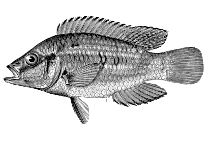
\includegraphics[width=0.38\textwidth]{fish}
%  \end{center}
%  \caption{Fish}
%\end{wrapfigure}
%\lipsum[7-8] % Dummy text
%
%%------------------------------------------------
%
%\subsubsection{Subsubsection 3} % Sub-sub-section
%
%\begin{description} % Numbered list example
%
%\item[First] \hfill \\
%\lipsum[9] % Dummy text
%
%\item[Second] \hfill \\
%\lipsum[10] % Dummy text
%
%\item[Third] \hfill \\
%\lipsum[11] % Dummy text
%
%\end{description} 

%----------------------------------------------------------------------------------------
%	MAJOR SECTION X - TEMPLATE - UNCOMMENT AND FILL IN
%----------------------------------------------------------------------------------------

%\section{Content Section}

%\subsection{Subsection 1} % Sub-section

% Content

%------------------------------------------------

%\subsection{Subsection 2} % Sub-section

% Content

%----------------------------------------------------------------------------------------
%	CONCLUSION
%----------------------------------------------------------------------------------------

%\section{Conclusion} % Major section
%asdsad \cite{deitel:1} adsads.
%\lipsum[12-13]



%----------------------------------------------------------------------------------------
%	BIBLIOGRAPHY
%----------------------------------------------------------------------------------------

\begin{thebibliography}{99} % Bibliography - this is intentionally simple in this template
	
\nocite{*} 

\printbibliography[heading=none]

%\bibitem[Figueredo and Wolf, 2009]{Figueredo:2009dg}
%Figueredo, A.~J. and Wolf, P. S.~A. (2009).
%\newblock Assortative pairing and life history strategy - a cross-cultural
%  study.
%\newblock {\em Human Nature}, 20:317--330.
 
\end{thebibliography}

%----------------------------------------------------------------------------------------

\end{document}